% Provenance (never printed): cycle 4 SVT/physique, "La planete Terre,
% l'environnement": the atmosphere, its structure and its layers, pressure
% and altitude, the ozone layer; see sources/book1/PROVENANCE.md. Book 1,
% grade 8, chapter 1.
% Vocabulary guard: owns the layers of the atmosphere (troposphere,
% tropopause, stratosphere, mesosphere, thermosphere), the environmental
% lapse rate and the ozone layer. Air pressure and the barometer are the
% physics books' (recalled), the composition of air and ozone the molecule
% the chemistry books'; "convection cell" is g8.2's and is not used here;
% adiabatic cooling is Book 2's.
\chapter{The Atmosphere}\label{ch:g8:the-atmosphere}

At a \omterm{def:g4:clouds-rain-snow:weather-station}{weather station}, just before the agreed hour, a meteorologist walks
out onto the grass holding a balloon filled with hydrogen or helium, about
\qty{1.5}{m} across. Below it, on a long string, hang a small orange
parachute and an instrument box of 60 to 80 grams: a \emph{radiosonde}.
She lets go. The balloon climbs about \qty{300}{m} every minute, and every
second the radiosonde radios down the pressure, the temperature, the
humidity and its position. As it rises, the balloon swells, until it is
6 to \qty{8}{m} across and bursts, often more than \qty{30}{km} up, two
hours after the launch. At the same hours of every day, the same scene
takes place at more than 800 stations around the world.
% ledger: nws:radiosonde

\begin{omfigure}
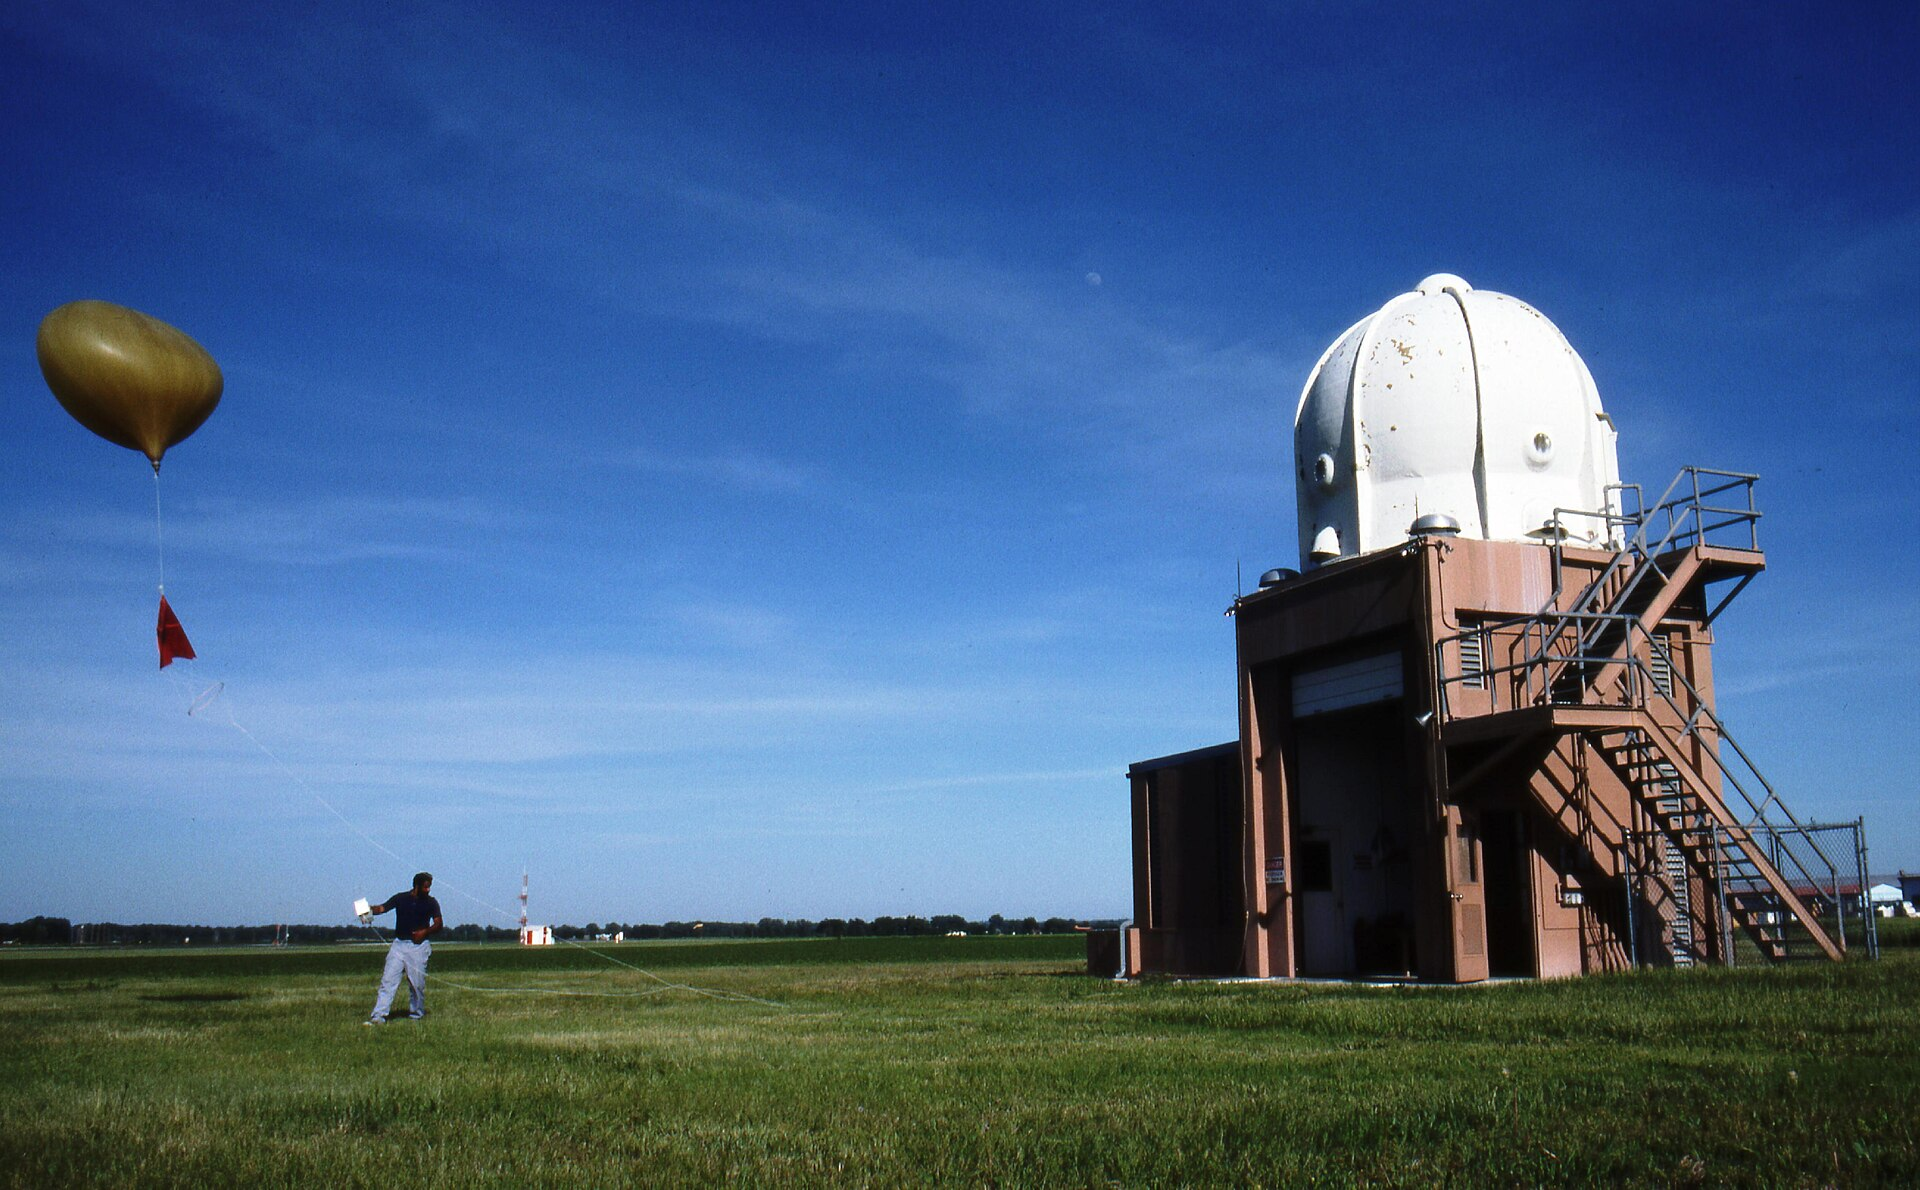
\includegraphics[width=0.78\linewidth]{images/book1/g8-radiosonde-launch.jpg}

{\small Launching a \omterm{def:g1:watching-the-weather:weather}{weather} balloon in Topeka, Kansas (United States):
the parachute (red) and the radiosonde hang below the balloon. Photograph
by Stephen Corfidi, NOAA/National Weather Service (public domain, via
Wikimedia Commons).}
% ledger: commons:radiosonde-launch
\label{fig:g8:the-atmosphere:launch}
\end{omfigure}

Why does the balloon swell as it rises? What does the radiosonde measure
on its way up, and why does the temperature not simply keep falling? Where
does the air end?

\begin{recall}
The \emph{atmosphere} is the layer of air around the Earth. Air presses
on everything it touches: this is \emph{air pressure}, measured with a
barometer (the physics books). \omterm{def:g1:watching-the-weather:weather}{Weather} services give it in hectopascals
(hPa); at \omterm{def:g4:world-physical-map:altitude}{sea level} it is about \qty{1013}{hPa}. Dry air is made of about
78~\% nitrogen and 21~\% oxygen, with a little argon, carbon dioxide and
other gases (the chemistry books). \omterm{def:g4:clouds-rain-snow:cloud}{Clouds} are made of tiny droplets of
water or crystals of ice (\cref{ch:g4:clouds-rain-snow}).
\end{recall}
% ledger: air:N2, air:O2, ussa76:sea-level

\section{A thin envelope}

Seen from the International Space Station, the atmosphere is a thin glowing
line along the edge of the Earth. Most of the air, and almost all the
\omterm{def:g4:clouds-rain-snow:cloud}{clouds}, are in its lowest few kilometres.
% ledger: commons:iss-sunset

\begin{omfigure}
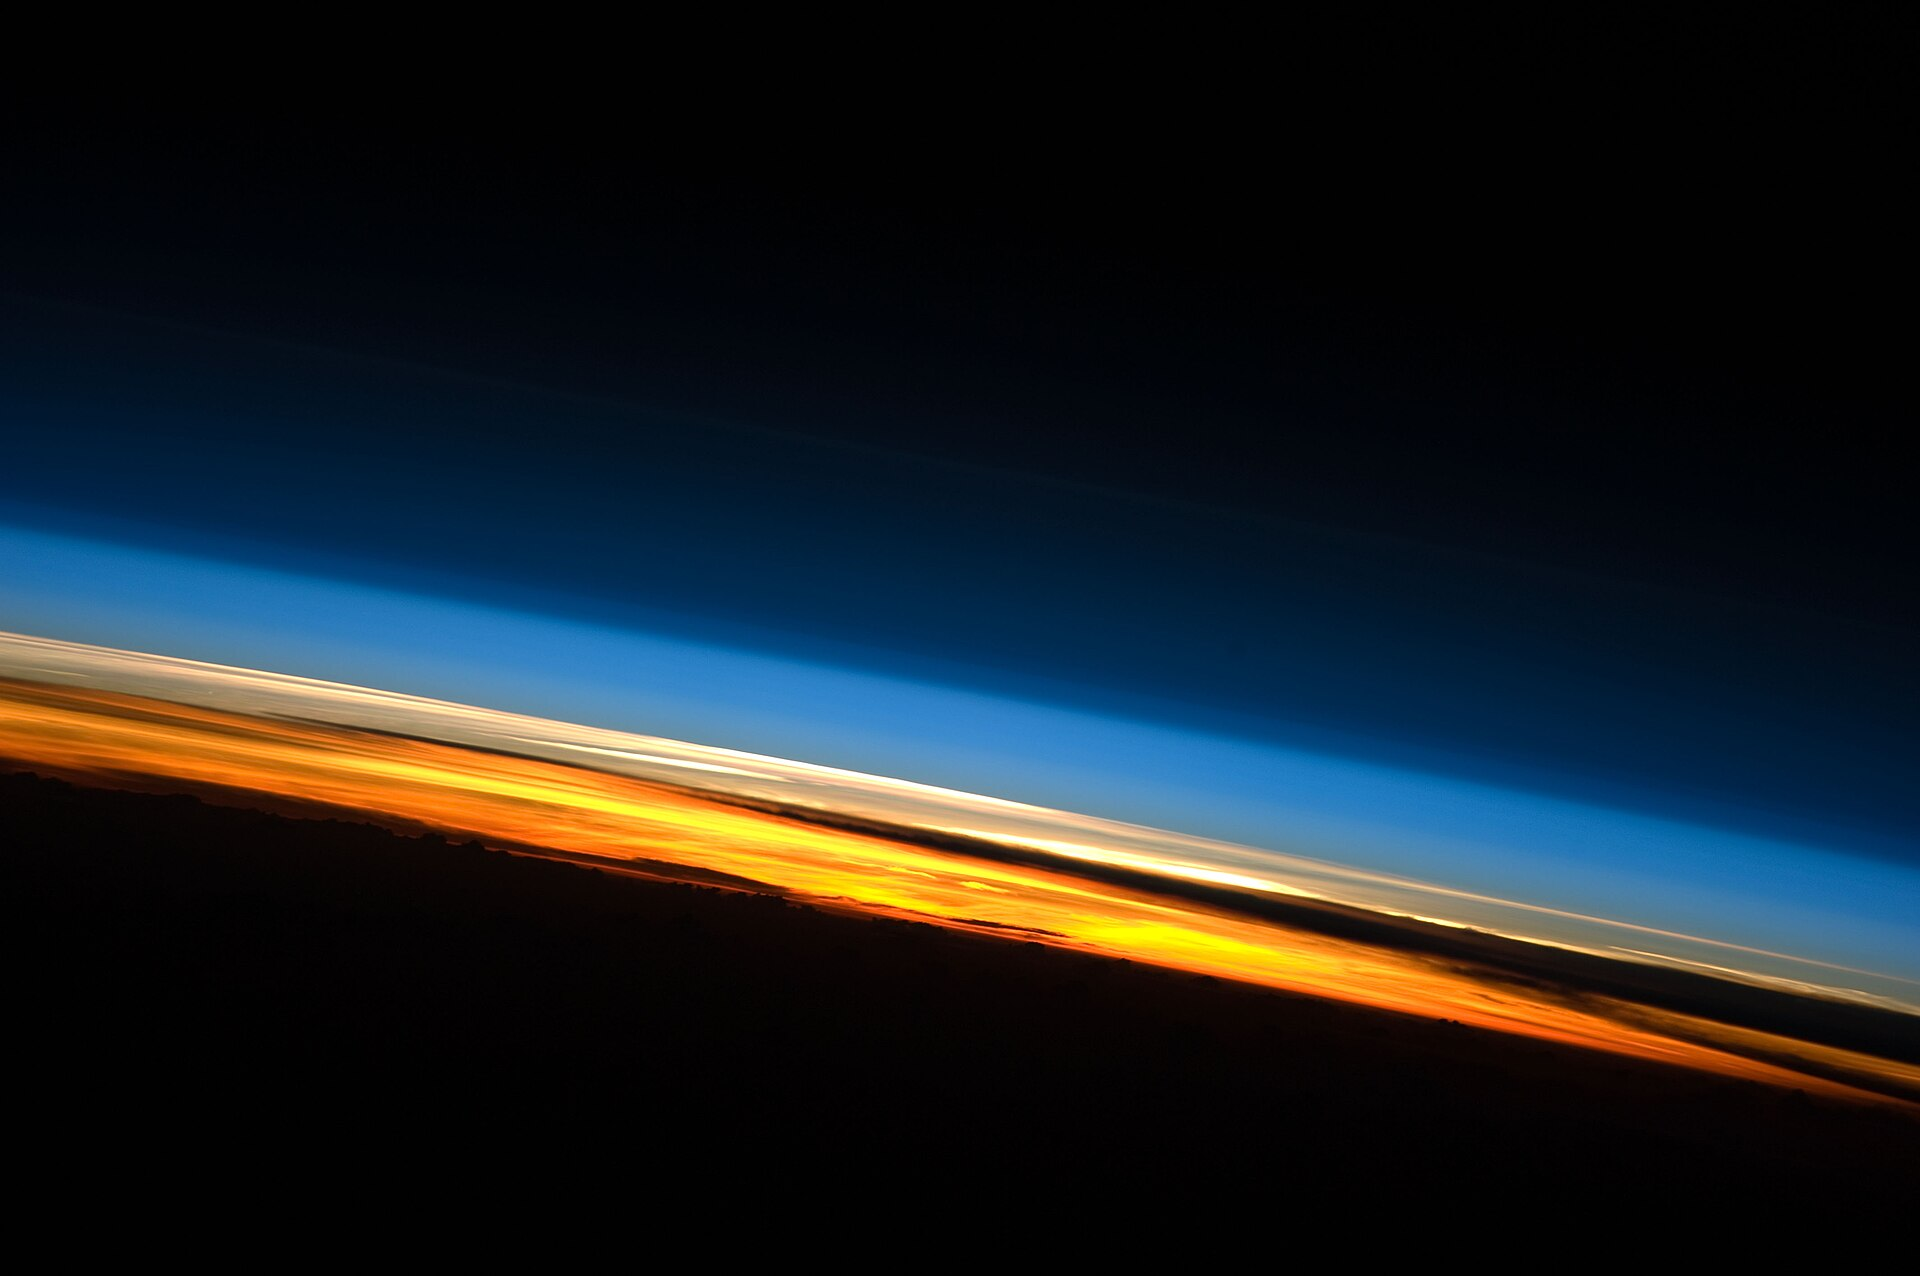
\includegraphics[width=0.78\linewidth]{images/book1/g8-iss-limb.jpg}

{\small The edge of the Earth at sunset, photographed from the
International Space Station above the Indian \omterm{def:g2:water-on-earth:ocean}{Ocean} on 14~June 2010. The
orange and yellow band is the lowest layer of the atmosphere, with its
dark \omterm{def:g4:clouds-rain-snow:cloud}{clouds}; above it come paler and then blue layers, fading into the
black of space. NASA photograph, ISS Expedition~23 (public domain, via
Wikimedia Commons).}
% ledger: commons:iss-sunset
\label{fig:g8:the-atmosphere:limb}
\end{omfigure}

There is no sharp top to the atmosphere: the air gets thinner and thinner
with height. By convention, space begins at about \qty{100}{km}. Compared
with the Earth's radius, \qty{6371}{km}, that is very little: $100 \div
6371 \approx 0.016$, less than 2~\% of the radius. On a \omterm{def:g3:continents-and-oceans:globe}{globe}
\qty{30}{cm} across, the whole atmosphere would be a film about
\qty{2}{mm} thick.
% ledger: ucar:layers, earth:Rmean

\begin{omfigure}
\begin{tikzpicture}[font=\footnotesize]
  % 1 cm = 100 km: the Earth's surface is a circle of radius 63.71 cm
  \def\R{63.71}
  \useasboundingbox (-6.9,-1.6) rectangle (6.9,1.0);
  \fill[blue!8] (0,-\R) ++(85:\R+1) arc (85:95:\R+1) -- ($(0,-\R)+(95:\R)$) arc (95:85:\R) -- cycle;
  \fill[omLithAlluv!70] (0,-\R) ++(85:\R) arc (85:95:\R) -- ++(0,-0.6) -- ($(0,-\R)+(85:\R)+(0,-0.6)$) -- cycle;
  \draw[black, line width=0.6pt] (0,-\R) ++(85:\R) arc (85:95:\R);
  \foreach \h/\c in {0.1102/omThm, 0.4938/omMeth, 0.86/omDef} \draw[\c, line width=0.5pt] (0,-\R) ++(85:\R+\h) arc (85:95:\R+\h);
  \draw[black!60, dashed] (0,-\R) ++(85:\R+1) arc (85:95:\R+1);
  \node[anchor=west, omThm] at (5.65,-0.14) {\qty{11}{km}};
  \node[anchor=west, omMeth] at (5.65,0.25) {\qty{49}{km}};
  \node[anchor=west, omDef] at (5.65,0.62) {\qty{86}{km}};
  \node[anchor=east, black!70] at (-5.65,0.75) {\qty{100}{km}};
  \node[anchor=north] at (0,-0.15) {the Earth's surface};
  \draw[|-|] (-5,-1.05) -- node[below] {\qty{1000}{km}} (5,-1.05);
\end{tikzpicture}

{\small A slice of the Earth and its atmosphere drawn to scale
(\qty{1}{cm} for \qty{100}{km}), up to \qty{100}{km}, the edge of
space (dashed). The coloured lines are the limits of the layers met
later in this chapter; the lowest layer, where all the \omterm{def:g1:watching-the-weather:weather}{weather} happens,
is barely a millimetre thick.}
% ledger: earth:Rmean, ucar:layers (limits: figdata/grade-8/standard_atmosphere.py main table)
\label{fig:g8:the-atmosphere:to-scale}
\end{omfigure}

\section{Pressure falls with altitude}

The air at the bottom of the atmosphere carries the weight of all the air
above it. The higher one climbs, the less air is left overhead, and the
lower the pressure. In the standard model of the atmosphere used by
meteorologists and engineers, the pressure is \qty{1013}{hPa} at \omterm{def:g4:world-physical-map:altitude}{sea
level}, half of that at about \qty{5.5}{km}, and a quarter at about
\qty{10.3}{km}.
% ledger: ussa76:sea-level, ussa76:layers (figdata/grade-8/standard_atmosphere.py main table: half_km 5.48, quarter_km 10.29)

Since the pressure measures the weight of the air above, the half-pressure
level is also the height below which half of all the air lies: half of
the atmosphere is squeezed into its lowest \qty{5.5}{km}. Below
\qty{11}{km} lies about 78~\% of the air, below \qty{30}{km} about 99~\%.
% ledger: (computed: figdata/grade-8/standard_atmosphere.py, share_below_11km 77.7, share_below_30km 98.82)

\begin{omfigure}
\begin{minipage}[t]{0.49\linewidth}\centering
\begin{tikzpicture}
\begin{axis}[width=6.6cm, height=7.6cm, xmin=0, xmax=1100, ymin=0, ymax=30,
  xlabel={pressure (hPa)}, ylabel={altitude (km)},
  tick label style={font=\scriptsize}, label style={font=\small},
  xtick={0,250,500,750,1000}, ytick={0,5,10,15,20,25,30}]
  \addplot[dashed, black!60] table {figdata/out/grade-8-standard_atmosphere-guides.dat};
  \addplot[omDef, line width=1.1pt] table[x=p_hPa, y=z_km] {figdata/out/grade-8-standard_atmosphere-pressure.dat};
  \addplot[only marks, mark=*, mark size=1.8pt, omThm, nodes near coords, point meta=explicit symbolic,
    every node near coord/.style={anchor=south west, font=\scriptsize, text=black}]
    table[x=p_hPa, y=z_km, meta=label] {figdata/out/grade-8-standard_atmosphere-levels.dat};
\end{axis}
\end{tikzpicture}

{\small Pressure against \omterm{def:g4:world-physical-map:altitude}{altitude}. The pressure is half its sea-level
value at about \qty{5.5}{km}, a quarter at about \qty{10.3}{km}.}
\end{minipage}\hfill
\begin{minipage}[t]{0.49\linewidth}\centering
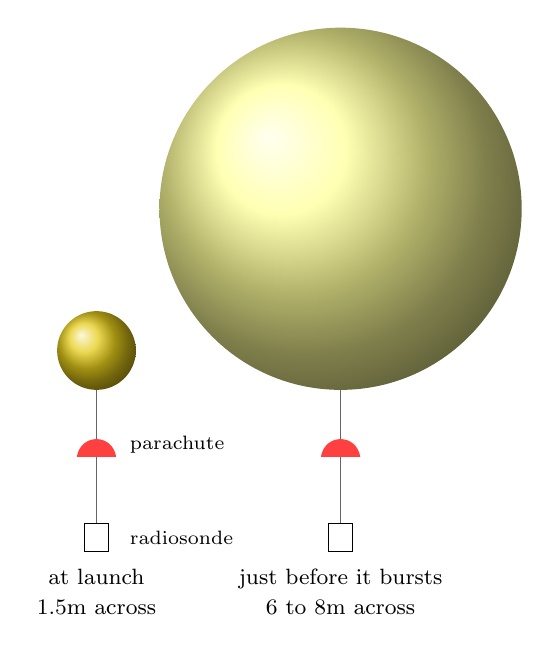
\begin{tikzpicture}[font=\footnotesize]
  % at launch: 1.5 m; at burst: about 7 m (drawn 1 cm for 1.5 m)
  \draw[black!60] (0,0.9) -- (0,2.6);
  \shade[ball color=yellow!60!brown] (0,3.1) circle (0.5);
  \fill[red!75] (-0.25,1.75) .. controls (-0.2,2.05) and (0.2,2.05) .. (0.25,1.75) -- cycle;
  \fill[white, draw=black] (-0.15,0.55) rectangle (0.15,0.9);
  \node[anchor=north] at (0,0.45) {at launch};
  \node[anchor=north] at (0,0.05) {\qty{1.5}{m} across};
  \begin{scope}[xshift=3.1cm]
    \draw[black!60] (0,0.9) -- (0,2.6);
    \shade[ball color=yellow!40!white] (0,4.9) circle (2.3);
    \fill[red!75] (-0.25,1.75) .. controls (-0.2,2.05) and (0.2,2.05) .. (0.25,1.75) -- cycle;
    \fill[white, draw=black] (-0.15,0.55) rectangle (0.15,0.9);
    \node[anchor=north] at (0,0.45) {just before it bursts};
    \node[anchor=north] at (0,0.05) {6 to \qty{8}{m} across};
  \end{scope}
  \node[anchor=west, font=\scriptsize] at (0.3,1.9) {parachute};
  \node[anchor=west, font=\scriptsize] at (0.3,0.72) {radiosonde};
\end{tikzpicture}

{\small The balloon swells as it climbs, because the air around it presses
less and less (balloons and parachutes to scale with each other, the
string shortened).}
% ledger: nws:radiosonde
\end{minipage}
% ledger: ussa76:sea-level, ussa76:layers (figdata/grade-8/standard_atmosphere.py parts pressure, levels, guides)
\label{fig:g8:the-atmosphere:pressure}
\end{omfigure}

Higher up, the pressure keeps falling, by about half again for every few
kilometres, so it soon becomes tiny. Powers of ten are the best way to
write it. At \qty{30}{km}, the pressure is about \qty{12}{hPa}, roughly
$10^{-2}$ of its sea-level value (one hundredth); at \qty{50}{km}, about
\qty{0.8}{hPa}, roughly $10^{-3}$; at \qty{80}{km}, about
\qty{0.01}{hPa}, roughly $10^{-5}$ of the sea-level pressure.
% ledger: ussa76:layers (figdata/grade-8/standard_atmosphere.py main table: p_30km 11.97, p_50km 0.798, p_80km 0.0105 hPa)

\begin{omfigure}
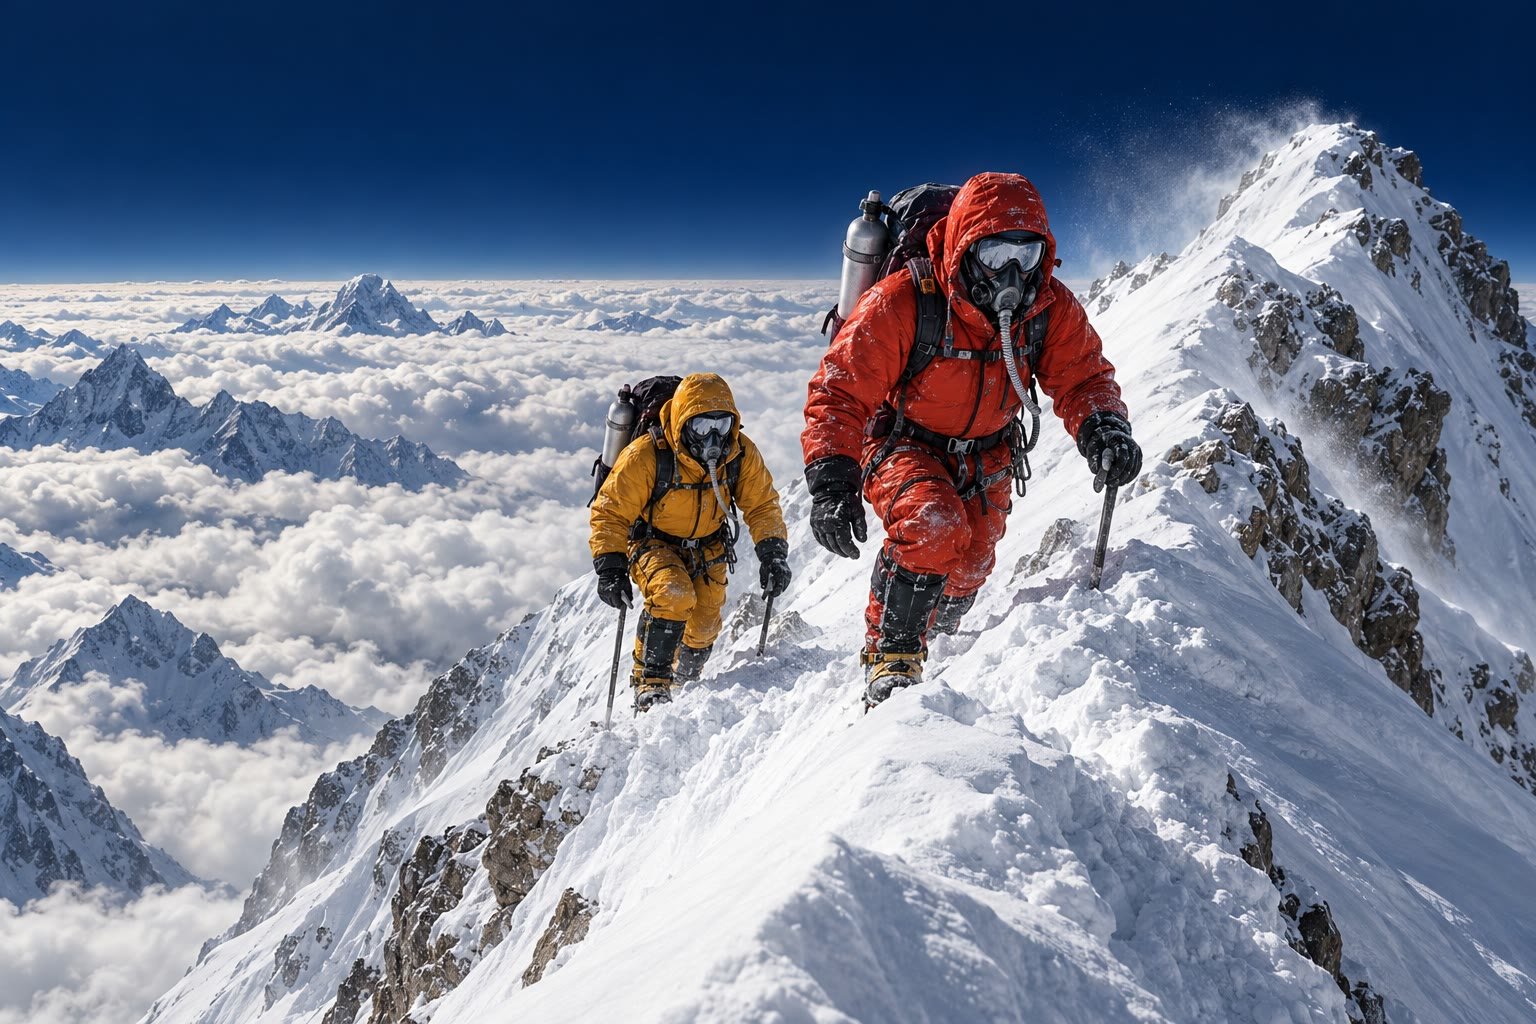
\includegraphics[width=0.5\linewidth]{images/book1/ai/g8-climbers.jpg}

{\small Climbers on a very high \omterm{def:g1:landscapes-around-us:landform}{mountain} carry bottles of oxygen. At
\qty{9}{km}, the pressure is less than a third of its sea-level value:
the air still holds 21~\% oxygen, but each breath takes in far less of
it (AI-generated illustration of a generic scene).}
% ledger: air:O2 (figdata/grade-8/standard_atmosphere.py: pressure at 9 km 308 hPa, 30 % of sea level)
\label{fig:g8:the-atmosphere:climbers}
\end{omfigure}

\section{Temperature and the layers}

Everyone who has climbed a \omterm{def:g1:landscapes-around-us:landform}{mountain} knows that the air gets colder with
height. The radiosondes show that this is true only in the lowest part of
the atmosphere. Higher up, the temperature stops falling, then rises, then
falls again, then rises once more. These changes divide the atmosphere into
layers.
% ledger: ucar:layers, ussa76:layers

\begin{omfigure}
\begin{tikzpicture}
\begin{axis}[width=10cm, height=9cm, xmin=-100, xmax=30, ymin=0, ymax=100,
  xlabel={temperature ($^\circ$C)}, ylabel={altitude (km)},
  tick label style={font=\scriptsize}, label style={font=\small},
  xtick={-100,-80,-60,-40,-20,0,20}, ytick={0,10,20,30,40,50,60,70,80,90,100}, axis on top]
  \addplot[fill=omSea!55, draw=none] table {figdata/out/grade-8-standard_atmosphere-band-troposphere.dat};
  \addplot[fill=omMeth!12, draw=none] table {figdata/out/grade-8-standard_atmosphere-band-stratosphere.dat};
  \addplot[fill=omSea!35, draw=none] table {figdata/out/grade-8-standard_atmosphere-band-mesosphere.dat};
  \addplot[fill=omThm!10, draw=none] table {figdata/out/grade-8-standard_atmosphere-band-thermosphere.dat};
  \addplot[omThm, line width=1.2pt] table[x=T_C, y=z_km] {figdata/out/grade-8-standard_atmosphere-temp.dat};
  \addplot[draw=none, nodes near coords, point meta=explicit symbolic,
    every node near coord/.style={anchor=west, font=\small\bfseries, text=black!75}]
    table[x=lx_C, y=mid_km, meta=name] {figdata/out/grade-8-standard_atmosphere-layers.dat};
  \draw[black!50, dashed] (axis cs:-100,11.02) -- (axis cs:30,11.02);
  \draw[black!50, dashed] (axis cs:-100,49.38) -- (axis cs:30,49.38);
  \draw[black!50, dashed] (axis cs:-100,86) -- (axis cs:30,86);
  \node[anchor=south east, font=\scriptsize] at (axis cs:17,11.02) {tropopause};
  \node[anchor=south east, font=\scriptsize] at (axis cs:29,49.38) {stratopause};
  \node[anchor=south east, font=\scriptsize] at (axis cs:29,86) {mesopause};
  \fill[omMeth!45] (axis cs:19,16) rectangle (axis cs:23,48);
  \node[anchor=east, font=\scriptsize, align=right] at (axis cs:18,30) {ozone\\layer};
\end{axis}
\end{tikzpicture}

{\small The temperature of the air against \omterm{def:g4:world-physical-map:altitude}{altitude}, from the ground to
\qty{100}{km}, in the standard atmosphere (an average for the middle
\omterm{def:g6:latitude-longitude:latitude}{latitudes}). The four layers are shaded; the green bar marks the height of
the \omterm{def:g8:the-atmosphere:ozone-layer}{ozone layer}.}
% ledger: ussa76:sea-level, ussa76:layers, ussa76:above-86, ucar:ozone (figdata/grade-8/standard_atmosphere.py parts temp, layers, band-*)
\label{fig:g8:the-atmosphere:temperature}
\end{omfigure}

\begin{definition}[The layers of the atmosphere]\label{def:g8:the-atmosphere:layers}
From the ground up, the atmosphere is divided into four layers by the
way its temperature changes with height:
\begin{itemize}
  \item the \emph{troposphere}\index{troposphere}, where the temperature
        falls with height and where almost all the \omterm{def:g1:watching-the-weather:weather}{weather} happens; its
        top is the \emph{tropopause}\index{tropopause};
  \item the \emph{stratosphere}\index{stratosphere}, where the temperature
        rises with height, up to about \qty{50}{km};
  \item the \emph{mesosphere}\index{mesosphere}, where the temperature
        falls again, up to about \qty{85}{km};
  \item the \emph{thermosphere}\index{thermosphere}, where the very thin
        air gets hotter and hotter with height.
\end{itemize}
\end{definition}
% ledger: ucar:layers, ussa76:layers

The \omterm{def:g8:the-atmosphere:layers}{troposphere} holds about 99~\% of the atmosphere's water vapour, so
nearly all \omterm{def:g4:clouds-rain-snow:cloud}{clouds}, \omterm{def:g4:clouds-rain-snow:precipitation}{rain} and \omterm{def:g4:clouds-rain-snow:precipitation}{snow} form in it. Its air is stirred all the
time. The top of the \omterm{def:g8:the-atmosphere:layers}{troposphere} is not at the same height everywhere: the
\omterm{def:g8:the-atmosphere:layers}{tropopause} is highest above the \omterm{def:g3:continents-and-oceans:equator}{equator}, where it can reach \qty{20}{km},
and lowest above the \omterm{def:g3:continents-and-oceans:poles}{poles}, where it can come down to \qty{7}{km} in
winter. It is also higher in summer than in winter. In the standard
atmosphere, an average for the middle \omterm{def:g6:latitude-longitude:latitude}{latitudes}, it lies at \qty{11}{km}.
% ledger: ucar:layers, ucar:tropopause, ussa76:layers

\begin{definition}[Environmental lapse rate]\label{def:g8:the-atmosphere:lapse-rate}
The \emph{environmental lapse rate}\index{environmental lapse rate} is the
rate at which the temperature of the air falls with height in the
\omterm{def:g8:the-atmosphere:layers}{troposphere}, in degrees Celsius per kilometre. It changes from day to day
and from place to place; the standard atmosphere uses an average of
\qty{6.5}{\degreeCelsius} per kilometre.
\end{definition}
% ledger: ussa76:layers

\begin{method}[Reading a temperature profile]\label{met:g8:the-atmosphere:profile}
\begin{enumerate}
  \item Find the \omterm{def:g4:world-physical-map:altitude}{altitude} on the vertical axis and go across to the
        curve; read the temperature below it.
  \item Where the curve leans to the left as it goes up, the air cools
        with height; where it leans to the right, the air warms with
        height; where it is vertical, the temperature does not change.
  \item The limits between layers are where the curve turns.
\end{enumerate}
\end{method}

\begin{example}[An airliner at cruising height]\label{ex:g8:the-atmosphere:airliner}
An airliner cruises at \qty{11}{km}, near the \omterm{def:g8:the-atmosphere:layers}{tropopause}. On the
profile, the temperature there is about \qty{-56}{\degreeCelsius}. With
the lapse rate: from \qty{15}{\degreeCelsius} at \omterm{def:g4:world-physical-map:altitude}{sea level}, the air cools
by $6.5 \times 11 = 71.5$ degrees, which gives $15 - 71.5 =
\qty{-56.5}{\degreeCelsius}$. On the pressure curve, the pressure is
about \qty{227}{hPa}, less than a quarter of the pressure on the ground:
the cabin has to be pressurised.
% ledger: ussa76:sea-level, ussa76:layers (figdata/grade-8/standard_atmosphere.py: T at 11 km -56.4 degC, p 227 hPa)
\end{example}

Above the \omterm{def:g8:the-atmosphere:layers}{tropopause}, in the \omterm{def:g8:the-atmosphere:layers}{stratosphere}, airliners find a calmer ride:
the air there gets warmer with height, so it is not stirred from below.
In the \omterm{def:g8:the-atmosphere:layers}{mesosphere} most meteors burn up, and at its top, near
\qty{86}{km}, is the coldest air of the whole atmosphere, about
\qty{-90}{\degreeCelsius}. In the \omterm{def:g8:the-atmosphere:layers}{thermosphere}, the Sun's X-rays and
ultraviolet light heat the very thin air to hundreds, at times
thousands, of degrees; yet there is so little air that it would not feel
warm. Many satellites orbit the Earth there.
% ledger: ucar:layers, ussa76:above-86

\section{The ozone layer}

The \omterm{def:g8:the-atmosphere:layers}{stratosphere} gets warmer with height because it absorbs part of the
Sun's light. The gas that does most of this is ozone, a form of oxygen
(its chemistry is in the chemistry books).

\begin{definition}[Ozone layer]\label{def:g8:the-atmosphere:ozone-layer}
The \emph{ozone layer}\index{ozone layer} is the part of the
\omterm{def:g8:the-atmosphere:layers}{stratosphere}, between about \qty{16}{km} and \qty{48}{km}, where about
90~\% of the atmosphere's ozone is found. It absorbs most of the Sun's
harmful ultraviolet light.
\end{definition}
% ledger: ucar:ozone

Even in the \omterm{def:g8:the-atmosphere:ozone-layer}{ozone layer}, ozone is rare: only 1 to 10 molecules in a
million. Yet together with oxygen, it stops between 95~\% and 99.9~\% of
the ultraviolet light that reaches the Earth, including the most harmful
kinds. The energy it absorbs is turned into heat, which is why the
temperature rises through the \omterm{def:g8:the-atmosphere:layers}{stratosphere}. Without the \omterm{def:g8:the-atmosphere:ozone-layer}{ozone layer}, the
ultraviolet light reaching the ground would harm living things.
% ledger: ucar:ozone

\begin{inthefield}[Following the weather balloons]
\omterm{def:g1:watching-the-weather:weather}{Weather} services publish the measurements of their radiosondes, often
as a chart of temperature against height for each launch. With an adult,
look for the soundings of the station nearest to you, made at 00:00 or
12:00 UTC. Find the height where the temperature stops falling: that is
the \omterm{def:g8:the-atmosphere:layers}{tropopause} on that day. Compare a winter sounding with a summer one.
\end{inthefield}
% ledger: nws:radiosonde, ucar:tropopause

\section{Exercises}

\begin{exercise}[$\star$]\label{exo:g8:the-atmosphere:1}
Match each layer with its description: \omterm{def:g8:the-atmosphere:layers}{troposphere}; \omterm{def:g8:the-atmosphere:layers}{stratosphere};
\omterm{def:g8:the-atmosphere:layers}{mesosphere}; \omterm{def:g8:the-atmosphere:layers}{thermosphere}. (a) The temperature rises with height and the
\omterm{def:g8:the-atmosphere:ozone-layer}{ozone layer} is found there. (b) Almost all the \omterm{def:g1:watching-the-weather:weather}{weather} happens there.
(c) The coldest air of the atmosphere is at its top. (d) The very thin
air is heated to hundreds of degrees; many satellites orbit there.
\end{exercise}

\begin{exercise}[$\star$]\label{exo:g8:the-atmosphere:2}
Use the temperature profile of the standard atmosphere. (a) What is the
temperature at \omterm{def:g4:world-physical-map:altitude}{sea level}? (b) At \qty{11}{km}? (c) At \qty{50}{km}?
(d) At \qty{86}{km}? (e) Between which \omterm{def:g4:world-physical-map:altitude}{altitudes} does the temperature
not change?
\end{exercise}

\begin{exercise}[$\star$]\label{exo:g8:the-atmosphere:3}
True or false? Correct the false sentences. (a) The temperature of the
air always falls with height. (b) Half of all the air lies below about
\qty{5.5}{km}. (c) The \omterm{def:g8:the-atmosphere:ozone-layer}{ozone layer} is in the \omterm{def:g8:the-atmosphere:layers}{troposphere}. (d) The
\omterm{def:g8:the-atmosphere:layers}{tropopause} is higher above the \omterm{def:g3:continents-and-oceans:equator}{equator} than above the \omterm{def:g3:continents-and-oceans:poles}{poles}.
\end{exercise}

\begin{exercise}[$\star$]\label{exo:g8:the-atmosphere:4}
In which layer is each of these? (a) A \omterm{def:g4:clouds-rain-snow:precipitation}{rain} \omterm{def:g4:clouds-rain-snow:cloud}{cloud}. (b) An airliner at
\qty{12}{km}. (c) A \omterm{def:g1:watching-the-weather:weather}{weather} balloon just before it bursts, at
\qty{32}{km}. (d) A meteor burning up at \qty{75}{km}.
\end{exercise}

\begin{exercise}[$\star\star$]\label{exo:g8:the-atmosphere:5}
On a summer day, it is \qty{20}{\degreeCelsius} at \omterm{def:g4:world-physical-map:altitude}{sea level}. Suppose the
air cools by \qty{6.5}{\degreeCelsius} per kilometre. (a) What is the
temperature at \qty{2}{km}? (b) At \qty{3}{km}? (c) At about what height
does the air reach \qty{0}{\degreeCelsius}? Round to one decimal.
\end{exercise}

\begin{exercise}[$\star\star$]\label{exo:g8:the-atmosphere:6}
A \omterm{def:g1:landscapes-around-us:landform}{mountain} hut stands at \qty{3000}{m}. A walker leaves a village at
\qty{500}{m} where it is \qty{18}{\degreeCelsius}. Using a lapse rate of
\qty{6.5}{\degreeCelsius} per kilometre: (a) How many kilometres does
the walker climb? (b) By how many degrees does the air cool? (c) What
temperature can the walker expect at the hut?
\end{exercise}

\begin{exercise}[$\star\star$]\label{exo:g8:the-atmosphere:7}
Suppose the pressure halves every \qty{5.5}{km}, starting from
\qty{1000}{hPa} at \omterm{def:g4:world-physical-map:altitude}{sea level}. (a) What is the pressure at \qty{5.5}{km}?
At \qty{11}{km}? At \qty{16.5}{km}? (b) The standard atmosphere gives
about \qty{506}{hPa}, \qty{227}{hPa} and \qty{96}{hPa} at these three
heights (for \qty{1013}{hPa} at \omterm{def:g4:world-physical-map:altitude}{sea level}). Is the halving rule good
near the ground? Higher up?
\end{exercise}

\begin{exercise}[$\star\star$]\label{exo:g8:the-atmosphere:8}
At \omterm{def:g4:world-physical-map:altitude}{sea level} the pressure is about \qty{1000}{hPa}, that is $10^3$~hPa.
(a) At \qty{30}{km} it is about \qty{10}{hPa}. Write this as a power of
ten, and say how many times smaller it is than at \omterm{def:g4:world-physical-map:altitude}{sea level}. (b) At
\qty{80}{km} it is about \qty{0.01}{hPa}. Write it as a power of ten.
(c) How many times smaller than at \omterm{def:g4:world-physical-map:altitude}{sea level} is it?
\end{exercise}

\begin{exercise}[$\star\star$]\label{exo:g8:the-atmosphere:9}
A \omterm{def:g1:watching-the-weather:weather}{weather} balloon is \qty{1.5}{m} across at launch and \qty{6}{m}
across when it bursts. (a) How many times wider is it when it bursts?
(b) Explain why it swells as it rises. (c) Why do \omterm{def:g1:watching-the-weather:weather}{weather} services hang
a parachute below it?
\end{exercise}

\begin{exercise}[$\star\star$]\label{exo:g8:the-atmosphere:10}
The \omterm{def:g8:the-atmosphere:layers}{tropopause} can reach \qty{20}{km} above the \omterm{def:g3:continents-and-oceans:equator}{equator} and come down to
\qty{7}{km} above the \omterm{def:g3:continents-and-oceans:poles}{poles} in winter. (a) How many times thicker is the
\omterm{def:g8:the-atmosphere:layers}{troposphere} above the \omterm{def:g3:continents-and-oceans:equator}{equator} in this case? Round to one decimal. (b) On
the standard profile, the \omterm{def:g8:the-atmosphere:layers}{tropopause} is at \qty{11}{km}. Is the standard
atmosphere closer to the \omterm{def:g3:continents-and-oceans:equator}{equator} or to the \omterm{def:g3:continents-and-oceans:poles}{poles}? (c) A pilot flies from
a polar region to the \omterm{def:g3:continents-and-oceans:equator}{equator} at a constant height of \qty{10}{km}. Is
the plane in the \omterm{def:g8:the-atmosphere:layers}{troposphere} or the \omterm{def:g8:the-atmosphere:layers}{stratosphere} at the start (in
winter)? At the end?
\end{exercise}

\begin{exercise}[$\star\star\star$]\label{exo:g8:the-atmosphere:11}
The share of all the air that lies below a height is $1 - p \div
p_0$, where $p$ is the pressure at that height and $p_0 =
\qty{1013}{hPa}$ the pressure at \omterm{def:g4:world-physical-map:altitude}{sea level}. (a) At \qty{5.5}{km}, $p
\approx \qty{506}{hPa}$: what share of the air lies below? (b) At
\qty{11}{km}, $p \approx \qty{227}{hPa}$. (c) At \qty{30}{km}, $p \approx
\qty{12}{hPa}$. Give the answers in per cent, to whole numbers. (d) What share of the air lies above \qty{30}{km}?
\end{exercise}

\begin{exercise}[$\star\star\star$]\label{exo:g8:the-atmosphere:12}
A school \omterm{def:g3:continents-and-oceans:globe}{globe} is \qty{30}{cm} across, so its radius, \qty{15}{cm},
stands for the Earth's radius, \qty{6371}{km}. (a) How many kilometres
does \qty{1}{cm} of the \omterm{def:g3:continents-and-oceans:globe}{globe} stand for? Round to the nearest kilometre.
(b) How thick, in millimetres, would the atmosphere up to \qty{100}{km}
be on this \omterm{def:g3:continents-and-oceans:globe}{globe}? (c) And the \omterm{def:g8:the-atmosphere:layers}{troposphere}, \qty{11}{km} thick? (d) A
sheet of paper is about \qty{0.1}{mm} thick. How many sheets would make
the \omterm{def:g8:the-atmosphere:layers}{troposphere} of the \omterm{def:g3:continents-and-oceans:globe}{globe}?
\end{exercise}

\section{Problem: Following a weather balloon}

\begin{problem}[{Weekend problem --- a weather balloon climbs through the
atmosphere; its temperatures show the layers, and its pressures show
where a quarter of the sea-level pressure is left}]
\label{pb:g8:the-atmosphere:1}
% ledger: nws:radiosonde; the table is the standard atmosphere, figdata/grade-8/standard_atmosphere.py part sonde
A radiosonde is launched from a station at \omterm{def:g4:world-physical-map:altitude}{sea level}. Its balloon rises
at about \qty{300}{m} per minute. The table gives the pressure and the
temperature it measures (the values of the standard atmosphere, rounded).

\begin{center}\small
\begin{tabular}{|l|*{8}{c|}}
\hline
\omterm{def:g4:world-physical-map:altitude}{altitude} (km) & 0 & 2 & 4 & 6 & 8 & 10 & 12 & 14 \\
\hline
pressure (hPa) & 1013 & 795 & 617 & 472 & 357 & 265 & 194 & 142 \\
\hline
temperature ($^\circ$C) & 15 & 2 & $-11$ & $-24$ & $-37$ & $-50$ & $-56$ & $-56$ \\
\hline
\hline
\omterm{def:g4:world-physical-map:altitude}{altitude} (km) & 16 & 18 & 20 & 22 & 24 & 26 & 28 & 30 \\
\hline
pressure (hPa) & 104 & 76 & 55 & 40 & 30 & 22 & 16 & 12 \\
\hline
temperature ($^\circ$C) & $-56$ & $-56$ & $-56$ & $-55$ & $-53$ & $-51$ & $-49$ & $-47$ \\
\hline
\end{tabular}
\end{center}

\noindent\textbf{Part I --- The climb.}\par\nopagebreak
\begin{enumerate}[beginpenalty=10000]
  \item How many metres does the balloon climb in 10 minutes?
  \item How long does it take to reach \qty{6}{km}? And \qty{30}{km}?
  \item The balloon bursts at \qty{30}{km}. How long has the flight
        lasted, in hours and minutes?
  \item Name the layer the balloon is in at \qty{8}{km}, and the layer it
        is in when it bursts.
\end{enumerate}

\noindent\textbf{Part II --- The temperature.}\par\nopagebreak
\begin{enumerate}[resume, beginpenalty=10000]
  \item By how many degrees does the temperature fall between the ground
        and \qty{10}{km}?
  \item What is the lapse rate in degrees per kilometre in this part of
        the climb?
  \item Between which \omterm{def:g4:world-physical-map:altitude}{altitudes} does the temperature stay the same?
        Where is the \omterm{def:g8:the-atmosphere:layers}{tropopause}?
  \item What happens to the temperature above \qty{20}{km}? Which gas
        explains it?
\end{enumerate}

\noindent\textbf{Part III --- The pressure.}\par\nopagebreak
\begin{enumerate}[resume, beginpenalty=10000]
  \item What is half of the sea-level pressure? Between which
        \omterm{def:g4:world-physical-map:altitude}{altitudes} is it reached?
  \item What is a quarter of the sea-level pressure? Round to the nearest
        hectopascal.
  \item Between which two \omterm{def:g4:world-physical-map:altitude}{altitudes} of the table is this quarter reached?
  \item The pressure falls by \qty{71}{hPa} between \qty{10}{km} and
        \qty{12}{km}. Supposing it falls evenly, at about what \omterm{def:g4:world-physical-map:altitude}{altitude}
        is the pressure a quarter of its sea-level value? Round to one
        decimal.
\end{enumerate}
\end{problem}
